\textbf{Problem 32.} \\
\hrule 

A certain brand of upright freezer is available in three different rated capacities: $16ft^3, 18ft^3$ and $20ft^3$. Let X = the rated capacity of a freezer of this brand sold at a certain store. Suppose X has the pmf given below.

\textbf{a. Compute $E(X), E(X^2)$, and $V(X)$}

\textbf{b. If the price of a freezer having capacity X is $70X - 650$, what is the expected price paid by the next customer to buy a freezer?}

\textbf{c. What is the variance of the price paid by the next customer?}

\textbf{d. Supose that although the rated capacity of a freezer is X, the actual capacity is $h(X) = X - .008X^2$. What is the expected actual capacity of the freezer purchased by the next customer? }

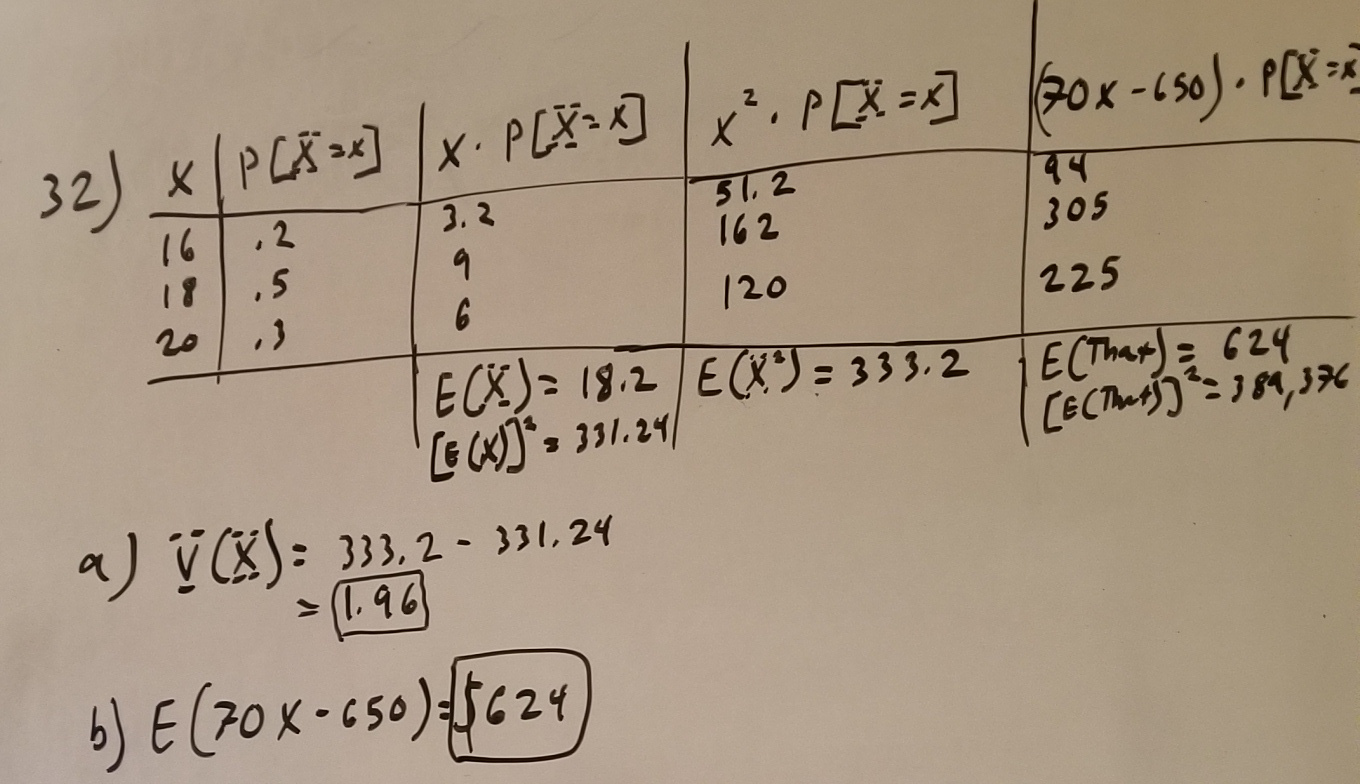
\includegraphics[scale=.25]{images/whw4/3.3.32A.jpg}

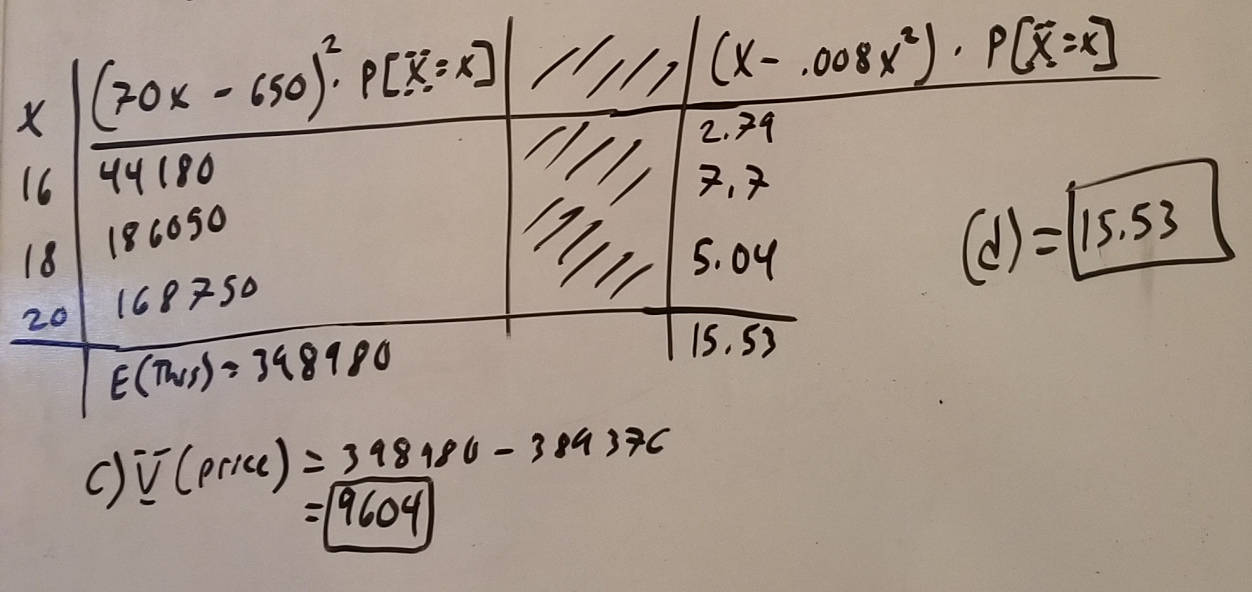
\includegraphics[scale=.25]{images/whw4/3.3.32B.jpg}